\documentclass[12pt]{article}
\usepackage{amsmath, amsfonts, amssymb}
\usepackage{mathtools}
\usepackage{graphicx}
\usepackage{xcolor}
\usepackage{lmodern}
\usepackage{fancyhdr}
\usepackage[most]{tcolorbox}
\usepackage{enumitem}

\definecolor{color1}{HTML}{941b0c}
\definecolor{color2}{HTML}{bc3908}
\definecolor{color3}{HTML}{f6aa1c}

\usepackage[font=small, labelfont=bf, justification=centering]{caption}
\usepackage[colorlinks=true, linkcolor=black, urlcolor=color2, citecolor=black]{hyperref}
\usepackage[a4paper, margin=1in]{geometry}

\title{\sffamily\bfseries{Balkan MO 1986 Solution}}
\author{Samuel de Araújo Brandão}
\date{August 2, 2025}

\pagestyle{fancy}
\fancyhf{}
\fancyhead[L]{\textbf{Balkan MO 1986 Solution}}
\fancyhead[R]{\textcolor{color2}{Samuel Brandão}, August 2, 2025}
\fancyfoot[C]{\thepage}
\setlength{\headheight}{14.5pt}

\renewcommand*\contentsname{\textsf{Contents}}

\tcbset{
  problembox/.style={
    enhanced,
    colback=white,
    colframe=color2,
    boxrule=1pt,
    arc=2mm,
    top=1pt,
    bottom=1pt,
    left=1pt,
    right=1pt,
    fonttitle=\sffamily\bfseries\color{white},
    colbacktitle=color2,
    title={#1}
  }
}

\begin{document}
  \maketitle
  A collection of Balkam MO 1986 solutions, inspired by Evan Chen’s style.

  All solutions were written by me while preparing for the International Mathematical Olympiad (IMO).

  If you spot any errors or have suggestions or comments, feel free to reach out!

  \tableofcontents

  \clearpage

  \section{\textsf{Problems}}
    \begin{enumerate}[label=\textbf{\arabic*.}]
      \item A line passing through the incenter $I$ of the triangle $ABC$ intersect
        its incircle at $D$ and $E$ and its circumcircle at $F$ and $G$, in such
        a way that the point $D$ lies between $I$ and $F$. Prove that:
        $DF \cdot EG \geq r^{2}$.

    \end{enumerate}

  \clearpage

  \section{\textsf{Solutions}}

    \subsection{Problem 1.}
      \begin{tcolorbox}[problembox={Problem statement}]
        A line passing through the incenter $I$ of the triangle $ABC$ intersect
        its incircle at $D$ and $E$ and its circumcircle at $F$ and $G$, in such
        a way that the point $D$ lies between $I$ and $F$. Prove that:
        $DF \cdot EG \geq r^{2}$.
      \end{tcolorbox}

      \begin{figure}[h]
        \centering
        \begin{minipage}{0.3\textwidth}
          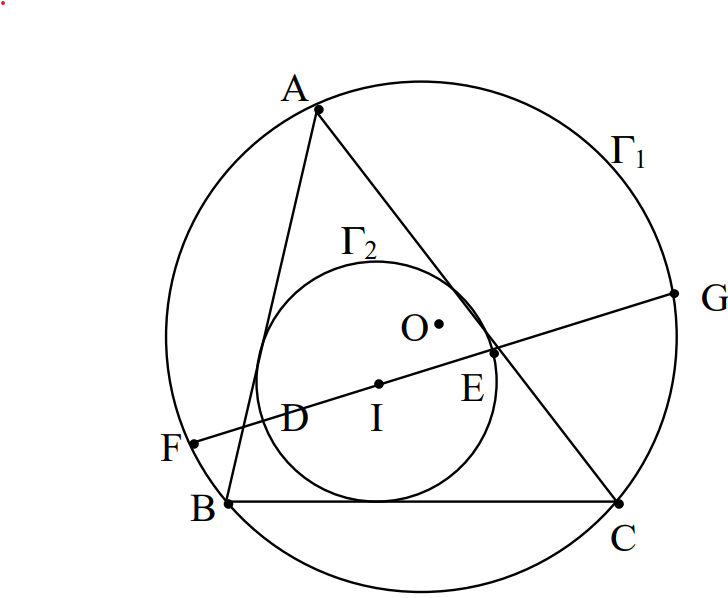
\includegraphics[width=\linewidth]{first.png}
          \caption{A figure illustrating the solution to the first problem. \href{https://www.obm.org.br/content/uploads/2017/01/eixos-2.pdf}{Source}}
        \end{minipage}
        \hfill
        \begin{minipage}{0.5\textwidth}
          \begin{align*}
            &DF \cdot EG = (IF - ID)(IG - IE) = (IF - r)(IG - r) \\
            &\text{where } r \text{ is the inradius. Hence} \\
            &IF \cdot IG - r(IF + IG) + r^2 = - Pot_{\Gamma_{1}} I - GFr + r^2 \\
            &= R^2 - IO^2 - GFr + r^2. \\
            &\text{Since the distance } IO \text{ between the incenter and} \\
            &\text{circumcenter satisfies } IO = \sqrt{R^2 - 2Rr}, \text{ it follows} \\
            &R^2 - IO^2 - GFr + r^2 = 2Rr - GFr + r^2 \Rightarrow 2Rr \\
            &- GFr + r^2 \geq r^2 \iff 2R r \geq GFr. \\
            &\text{This inequality holds since } GF \text{ is a chord of } \Gamma_1. \\
            &DF \cdot EG = r^2 \iff 2Rr = GFr.
          \end{align*}
        \end{minipage}
      \end{figure}

    \clearpage

    \subsection{Problem 2.}
    
    \clearpage

    \subsection{Problem 3.}

    \clearpage

    \subsection{Problem 4.}

  \clearpage

  \section{\textsf{References}}
    This document was made possible thanks to the help and inspiration of the following resource:
    \renewcommand{\refname}{\vspace{-2em}}
    \begin{thebibliography}{9}
      \bibitem{obm}
      OBM - Olimpíada Brasileira de Matemática.
      \textit{Potência de Ponto, Eixo Radical, Centro Radical e Aplicações}, 2017.
      Available in: \url{https://www.obm.org.br/content/uploads/2017/01/eixos-2.pdf}
    \end{thebibliography}
\end{document}
